\documentclass[12pt]{report}
\usepackage[utf8]{inputenc}
\usepackage[margin=1.2in]{geometry}
\usepackage{graphicx}
\usepackage{float}
\usepackage{subcaption}
\usepackage{amsmath}
\usepackage{amssymb}
\usepackage{ulem}
\usepackage{bm}
\usepackage{framed}
\usepackage{xcolor}
\usepackage{ragged2e}
\usepackage{color}
\usepackage{soul}
\usepackage{cancel}
\graphicspath{ {images/} }
\setlength{\parskip}{1em}
\allowdisplaybreaks


\usepackage{titling}
\newcommand{\subtitle}[1]{%
	\posttitle{%
		\par\end{center}
	\begin{center}\large#1\end{center}
	\vskip0.5em}%
}

\newenvironment{blueframed}[1][blue]
{\def\FrameCommand{\fboxsep=\FrameSep\fcolorbox{#1}{white}}%
\MakeFramed {\advance\hsize-\width \FrameRestore}}
{\endMakeFramed}

\newenvironment{spmatrix}[1]
{\def\mysubscript{#1}\mathop\bgroup\begin{bmatrix}}
{\end{bmatrix}\egroup_{\textstyle\mathstrut\mysubscript}}


\title{Tutorial 2}
\author{Quang Bui}
\subtitle
{
	\textbf{keywords}: cross sectional data, time series data, histogram, summary statistics, scatter plot, confidence interval of population mean, logarithmic transformation, trends, seasonality
	
	\textbf{estimated reading time}: 34 minutes
}
\date{July 31, 2018}

\begin{document}
	
\maketitle

\section*{Question 1}

\justify
\begin{blueframed}
	\textcolor{blue}{\textbf{Background}}
	\vspace{-\baselineskip}
	\justify
	\textcolor{blue}{\underline{Types of data sets} \begin{itemize}
			\item A \textit{cross-sectional} data set consists of a sample of individuals, households, firms, cities, countries, or a variety of other units, taken at a given point in time. For example, 40 countries' wine consumption level, GDP per capita, and infant mortality in 2015.
			\item A \textit{time-series} data set consists of observations on a variable or several variables over time. For example, Australia's wine consumption level, GDP per capita, and infant mortality every year from 2005 to 2015.
			\item A \textit{panel} data set consists of a time series of \textit{each} cross-sectional member in the data set. For example, 40 countries' wine consumption level, GDP per capita, and infant mortality every year from 2005 to 2015.
	\end{itemize}}
\end{blueframed}

\noindent EViews workfile: \textit{A random sample of countries.wf1}

\noindent \textit{A random sample of countries.wf1} contains data on 40 randomly selected countries from the population of all countries. Since this data set was capture at a single time period, we call this a cross-sectional data set. The variables in this data set include:
\begin{align*}
ccode &- country\ code \\
gdppc &- 2015\ GDP\ per\ capita\ measured\ in\ USD\ \&\ adjusted\ for\ purchasing\ power\ difference \\
infmort &- 2015\ infant\ mortality\ measured\ in\ number\ of\ deaths\ per\ 1000\ lives 
\end{align*}

\noindent To view the data set, select and highlight $ccode$, $gdppc$, and $infmort$ then,
$$Right\ click \to Open \to as\ Group$$
\begin{figure}[H]
	\centerline{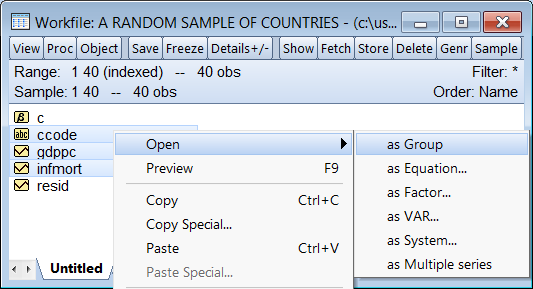
\includegraphics{2018sem2_q1}}
\end{figure}
\begin{figure}[H]
	\centerline{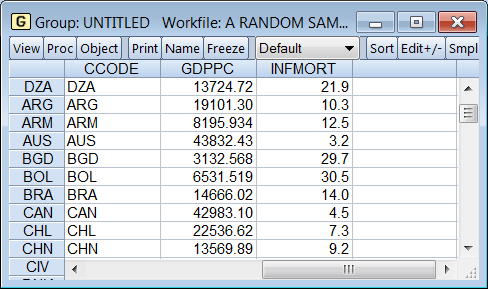
\includegraphics{2018sem2_q1_1}}
\end{figure}

\noindent \textcolor{red}{1. Obtain the summary statistics and histogram of $gdppc$. Discuss what you can learn from the histogram and summary statistics. If you had a different set of 40 countries, would the summary statistics be the same?}

\justify
\begin{blueframed}
	\textcolor{blue}{\textbf{Background}}
	\vspace{-\baselineskip}
	\justify
	\textcolor{blue}{\underline{Population parameters and sample statistics}}
	
	\noindent \textcolor{blue}
	{
		Population parameters describe the true behaviour of the population considered. For example, the population mean of 2015 GDP per capita is a value that describes the average GDP per capita in 2015 in the population of all countries. Without population data (and this is often the case in practice), we cannot calculate population parameters and the true behaviour of the population is unknown.}
\end{blueframed} 
\begin{blueframed} \textcolor{blue}{\vspace{-\baselineskip} \noindent Greek letters are used to denote population parameters, \begin{itemize}
			\item Population mean, $\mu$
			\item Population standard deviation, $\sigma$
			\item Population variance, $\sigma^2$
			\item Population intercept coefficient, $\beta_0$
			\item Population slope coefficient of variable $j$, $\beta_j$
			\item etc.
		\end{itemize} Since population data is often unavailable in practice, we cannot calculate population parameters and the true behaviour of the population is unknown. In practice, we draw a random sample from the population (we hope this is representative of the population) and use this sample to make inferences and learn about the true behaviour of the population. For example, suppose it were not feasible to gather data on the 2015 GDP per capita of every country, so instead, we obtain a sample of 40 randomly selected countries, \begin{figure}[H]
		\centerline{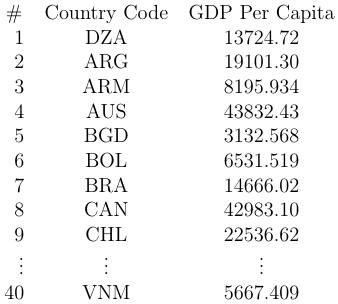
\includegraphics{2018sem2_q1_14}}
	\end{figure}
\vspace{-\baselineskip} \noindent With this sample, we can obtain summary statistics of the 2015 GDP per capita (among other things). Summary statistics, which summarise the central tendency, variability, and shape of a variable, include sample statistics like the sample mean, sample median, sample standard deviation, sample maximum \& sample minimum and are estimates of the population mean, population median, population standard deviation, population maximum \& population maximum.}
\end{blueframed}
\begin{blueframed} \noindent \textcolor{blue}{\noindent Sample statistics are random variables because they vary from sample to sample e.g. with a different sample of 40 countries, the sample mean changes. In fact, if we applied repeated sampling, we would have a `sample of sample means' and this too would have its own set of summary statistics.}
\end{blueframed}

%%%%%%%%%% TABLE OBJECT %%%%%%%%%%
%\begin{table}[!htbp]
%	\centering
%	\begin{tabular}{lrr}
%		\multicolumn{1}{c}{\#}&\multicolumn{1}{c}{Country Code}&\multicolumn{1}{c}{GDP Per Capita}\\
%		\multicolumn{1}{r}{$1$}&\multicolumn{1}{c}{DZA}&\multicolumn{1}{c}{$13724.72$}\\
		%\multicolumn{1}{r}{$2$}&\multicolumn{1}{c}{ARG}&\multicolumn{1}{c}{$19101.30$}\\
		%\multicolumn{1}{r}{$3$}&\multicolumn{1}{c}{ARM}&\multicolumn{1}{c}{$8195.934$}\\
		%\multicolumn{1}{r}{$4$}&\multicolumn{1}{c}{AUS}&\multicolumn{1}{c}{$43832.43$}\\
		%\multicolumn{1}{r}{$5$}&\multicolumn{1}{c}{BGD}&\multicolumn{1}{c}{$3132.568$}\\
		%\multicolumn{1}{r}{$6$}&\multicolumn{1}{c}{BOL}&\multicolumn{1}{c}{$6531.519$}\\
		%\multicolumn{1}{r}{$7$}&\multicolumn{1}{c}{BRA}&\multicolumn{1}{c}{$14666.02$}\\
		%\multicolumn{1}{r}{$8$}&\multicolumn{1}{c}{CAN}&\multicolumn{1}{c}{$42983.10$}\\
		%\multicolumn{1}{r}{$9$}&\multicolumn{1}{c}{CHL}&\multicolumn{1}{c}{$22536.62$}\\
		%\multicolumn{1}{r}{\vdots}&\multicolumn{1}{c}{$\vdots$}&\multicolumn{1}{c}{$\vdots$}\\
%		\multicolumn{1}{r}{$40$}&\multicolumn{1}{c}{VNM}&\multicolumn{1}{c}{$5667.409$}\\
%	\end{tabular}
	%\caption{Add your caption here.}
	%\label{tab:}
%\end{table}



\noindent To obtain the summary statistics and histogram of $gdppc$,
\begin{figure}[H]
	\centerline{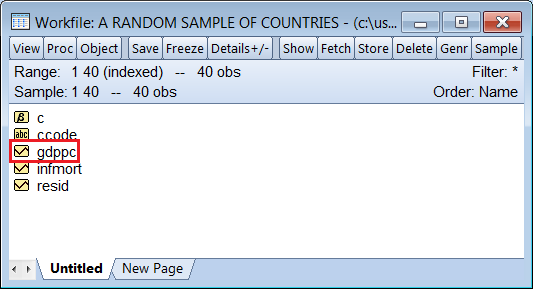
\includegraphics{2018sem2_q1_2}}
\end{figure}
\noindent double-click $gdppc$ then, $$View \to Descriptive\ Statistics\ \&\ Tests \to Histogram\ and\ Stats$$
\begin{figure}[H]
	\centerline{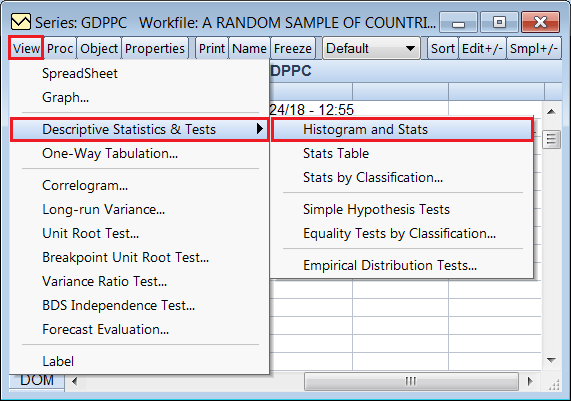
\includegraphics{2018sem2_q1_3}}
\end{figure}
\begin{figure}[H]
	\centerline{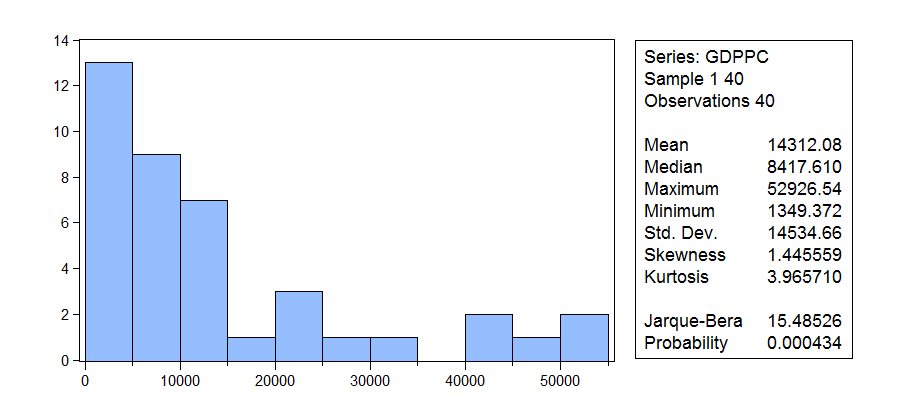
\includegraphics{2018sem2_q1_4}}
\end{figure}
\begin{itemize}
	\item GDP per capita has a positively skewed (right-tailed) distribution.
	\item The sample mean of GDP per capita is much higher than the sample median $$sample\ mean\ = \$14312.08 > sample\ median\ = \$8417.61$$ which suggests huge inequality among these 40 countries i.e. some countries in our random sample have a particularly high GDP per capita relative to the rest, which causes the mean to be greater than the median.
	\item The minimum GDP per capita is \$1349.37, which is less than 1/6 of the median in this sample and translates to \$3.70 per day per person. (The more descriptive your explanation, the better. Since GDP per capita is skewed, the median is a better measure of the central tendency of GDP per capita than the mean, so we compare the minimum against the median instead of the mean.)
	\item The maximum GDP per capita is \$52926.54, which is more than 6 times the median in this sample and translates to \$145 per day per person.
\end{itemize}
\noindent If we had 40 different countries, the summary statistics would change. This means that each sample statistic e.g. sample mean, sample median, sample maximum, sample minimum, sample standard deviation, etc. are random variables i.e. their values are uncertain and differ from sample to sample.



\newpage
\noindent \textcolor{red}{2. Using the sample average (mean) and sample standard deviation, compute the 95\% confidence interval for the population mean of $gdppc$. The confidence interval is given by equation [C.23] in Appendix C of the textbook. It is okay to use the rule of thumb given by equation [C.26] in the textbook. Explain what the confidence interval shows. The average $gdppc$ for all countries in the WDI data base in 2015 is \$17406. Does your confidence interval contain this value?}

\justify
\begin{blueframed}
	\textcolor{blue}{\textbf{Background}}
	\vspace{-\baselineskip}
	\justify
	\textcolor{blue}{\underline{Point Estimate of Population Mean}}
	
	\noindent \textcolor{blue}
	{
		The sample mean is a point estimate of the population mean and of course, there are many estimators of the population mean, e.g. randomly picking a number from the sample and using this as an estimate of the population mean, but this is clearly a poor estimator of the population mean. Point estimates alone do not inform us about the precision with which we have estimated the population parameter. \begin{align*}
		 \overline{gdppc} &= 14312.08 \\
		 \mu &=\ ???
		\end{align*} \underline{Confidence Interval of Population Mean}
	}
	
	\noindent \textcolor{blue}
	{
		Unlike a point estimator, a confidence interval provides a range of values $$[\dots,\dots]$$ so that we have a sense of what the population parameter might be, and the precision with which we have estimated it. \\ \\ For example, a 95\% confidence interval of the population mean tells us that we are 95\% confident that the population mean will lie between this range of values. If you can be 95\% confident that the population mean lies between a narrow range of values, $$[14302.18,14322.08]$$ then you would be very confident about your point estimate of the population mean (think about the formula of the confident interval, and what causes the width of the interval to increase/decrease). 
	}
\end{blueframed}

\noindent Using the simple rule of thumb for a 95\% confidence interval of the population mean, 
\begin{align*}
	[&\overline{gdppc} \pm 2 \times se(\overline{gdppc})] \\
	[&\overline{gdppc} - 2 \times se(\overline{gdppc}), \overline{gdppc} + 2 \times se(\overline{gdppc})] \\
	%[&\overline{gdppc} - 2 \times standard\ error_{\overline{gdppc}}, \overline{gdppc} + 2 \times standard\ error_{\overline{gdppc}}] \\
	[&\overline{gdppc} - 2 \times \dfrac{sample\ std.dev_{gdppc}}{\sqrt{n}}, \overline{gdppc} + 2 \times \dfrac{sample\ std.dev_{gdppc}}{\sqrt{n}}] \\
	[&14312.08 - 2 \times \dfrac{14534.66}{\sqrt{40}}, 14312.08 + 2 \times \dfrac{14534.66}{\sqrt{40}}] \\
	[&9716,18908]
\end{align*}

\noindent To interpret this confidence interval, we say that there is a 95\% chance that the 2015 population mean of GDP per capita lies between \$9716 and \$18908. It is incorrect to say that ``95\% of the time, the 2015 population mean of GDP per capita will lie between \$9716 and \$18908".

\noindent This confidence interval contains \$17406, which is the mean GDP per capita per annum in 2015 for all countries (this is a population mean so it is constant and does not change). Since the confidence interval depends on the sample mean and sample standard deviation, which differ from sample to sample, a different sample of 40 countries results in a slightly different confidence interval. 

%\noindent Note: The confidence interval of the population mean is only reliable when the sample mean follows a normal distribution. For a sufficiently large sample size ($n>30$), the sample mean will be close to normal. (More on this next time.)

\newpage
\noindent \textcolor{red}{3. We want to explore the association of infant mortality and GDP per capita. What kind of graph can give us an insight into the nature of this relationship? Based on this graph, are infant mortality and GDP per capita positively or negatively correlated? Is their relationship linear?}

\noindent Scatter plots can give us an insight into the nature of the relationship between two variables. To obtain a scatter plot of infant mortality (y-axis) against GDP per capita (x-axis),
$$Quick \to Graph \dots$$
\begin{figure}[H]
	\centerline{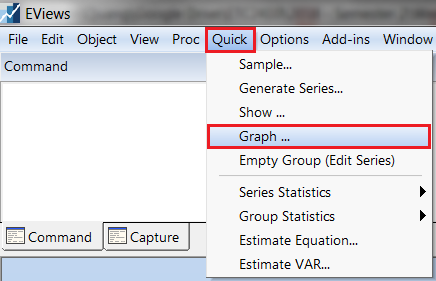
\includegraphics{2018sem2_q1_5}}
\end{figure}
\vspace{-\baselineskip} \noindent in the \textit{Series List} window, type the variable to go on the x-axis followed by the variable to go on the y-axis,
\begin{figure}[H]
	\centerline{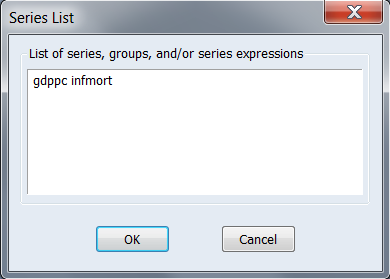
\includegraphics{2018sem2_q1_6}}
\end{figure}
\vspace{-\baselineskip} \noindent Under \textit{Specific}, select \textit{Scatter} and press \textit{OK},
$$Specific:Scatter \to OK$$
\begin{figure}[H]
	\centerline{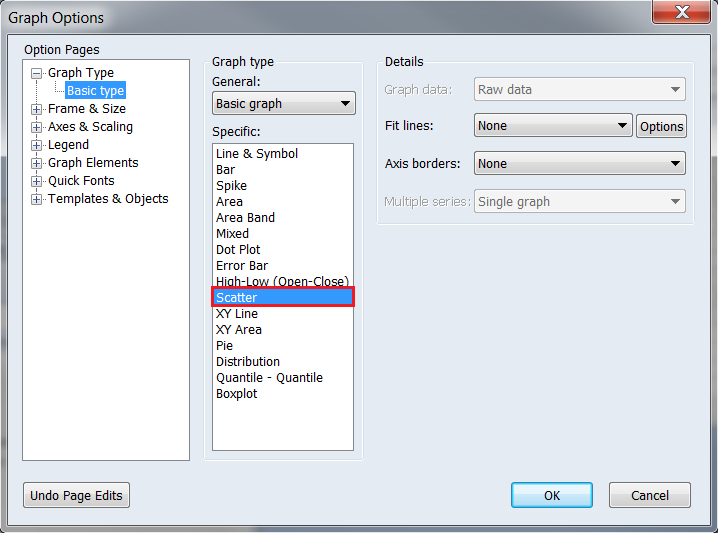
\includegraphics{scat3}}
\end{figure}
\vspace{-\baselineskip}	
\begin{figure}[H]
	\centerline{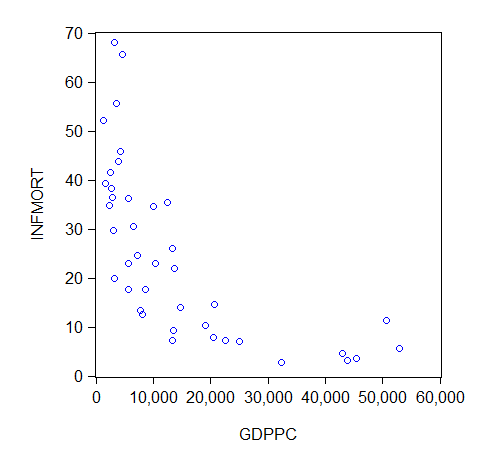
\includegraphics{2018sem2_q1_7}}
\end{figure}
\vspace{-\baselineskip}	\noindent The scatter plot shows that infant mortality and GDP per capita are negatively related but this relationship is non-linear.

\noindent \textcolor{red}{4. Generate the logarithmic transformation of $gdppc$ and $infmort$. Use the label $lgdppc$ for the natural logarithm of $gdppc$ and $linfmort$ for the natural logarithm of $infmort$. Note: In EViews, $log(X)$ calculates the natural logarithm of $X$. EViews does not recognise $ln(X)$. Explore the association between $linfmort$ and $lgdpcc$ with the aid of an appropriate graph. Compare and contrast it with what you got in the preious part.}

\noindent To generate the variables $lgdppc$, which are the natural logarithm of $gdppc$, in EViews,
$$Genr \to Enter\ equation:lgdppc = log(gdppc) \to OK$$
\begin{figure}[H]
	\centerline{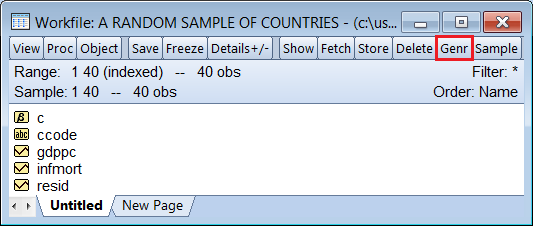
\includegraphics{2018sem2_q1_8}}
\end{figure}
\vspace{-\baselineskip}
\begin{figure}[H]
	\centerline{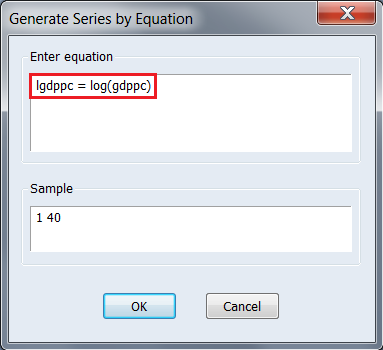
\includegraphics{2018sem2_q1_9}}
\end{figure}
\vspace{-\baselineskip} \noindent To generate the variables $linfmort$, which are the natural logarithm of  $infmort$, in EViews,
$$Genr \to Enter\ equation:linfmort = log(infmort) \to OK$$
\begin{figure}[H]
	\centerline{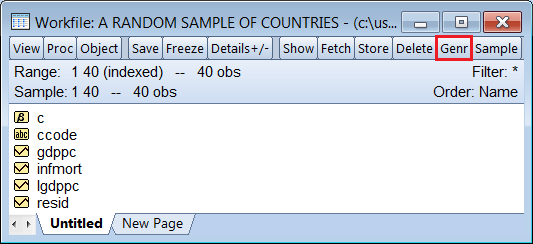
\includegraphics{2018sem2_q1_10}}
\end{figure}
\vspace{-\baselineskip}
\begin{figure}[H]
	\centerline{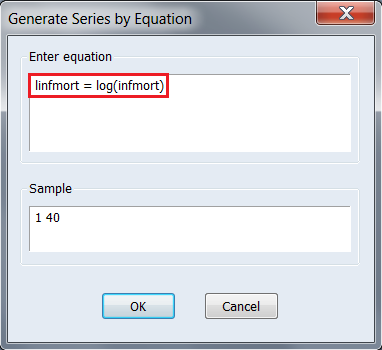
\includegraphics{2018sem2_q1_11}}
\end{figure}
\vspace{-\baselineskip}
\begin{figure}[H]
	\centerline{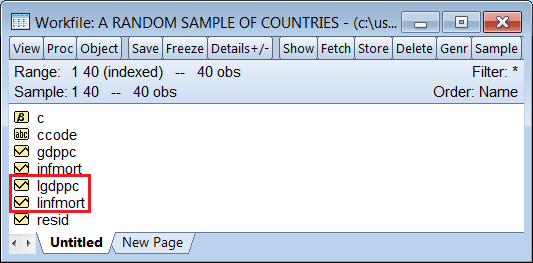
\includegraphics{2018sem2_q1_12}}
\end{figure}
\vspace{-\baselineskip}

\newpage
\noindent To obtain a scatter plot of $linfmort$ (y-axis) against $lgdppc$ (x-axis),
$$Quick \to Graph \dots$$
\begin{figure}[H]
	\centerline{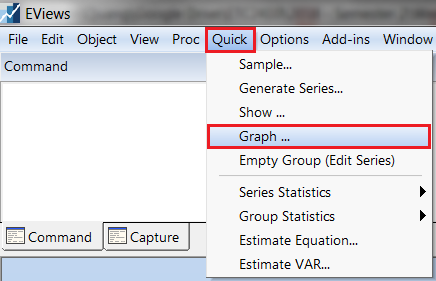
\includegraphics{2018sem2_q1_5}}
\end{figure}
\vspace{-\baselineskip} \center $Series\ List: lgdppc\ linfmort$
\begin{figure}[H]
	\centerline{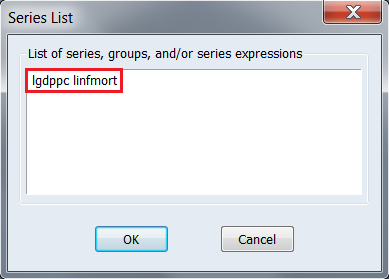
\includegraphics{2018sem2_q13}}
\end{figure}
\vspace{-\baselineskip} \justify \noindent Under \textit{Specific}, select \textit{Scatter} and press \textit{OK},
$$Specific:Scatter \to OK$$
\begin{figure}[H]
	\centerline{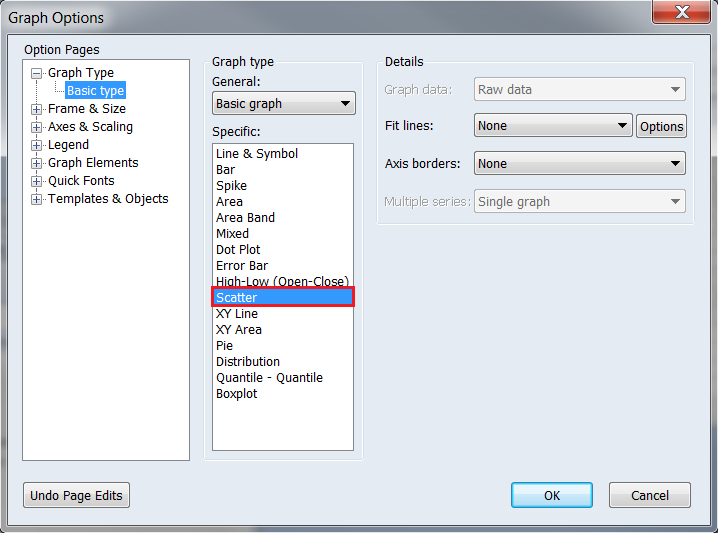
\includegraphics{scat3}}
\end{figure}
\vspace{-\baselineskip}	
\begin{figure}[H]
	\centerline{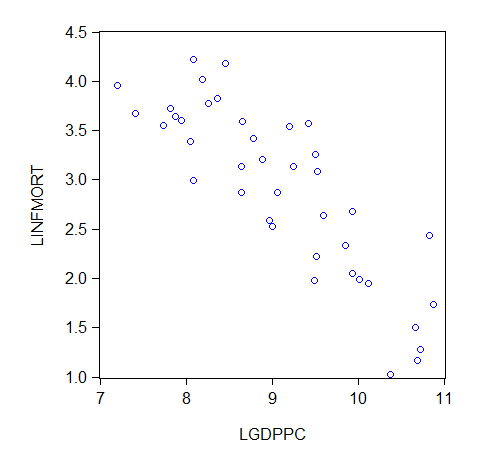
\includegraphics{scatter}}
\end{figure}
\vspace{-\baselineskip}	\noindent Unlike $infmort\ \&\ gdppc$, which have a non-linear relationship, the log of infant mortality $\&$ log of GDP per capita have a stronger linear relationship. We learn from this exercise that we may have to transform the raw data before we model their relationship in a model with linear parameters.

\noindent Consider the following simple linear regression models,
\begin{align}
linfmort &= \beta_0 + \beta_1 lgdppc + u \\
infmort &= \alpha_0 + \alpha_1 gdppc + v
\end{align}
\noindent Both models are linear in the parameters, but $(1)$ specifies a linear relationship between log of infant mortality and log of GDP per capita, while $(2)$ specifies a linear relationship between infant mortality and GDP per capita. Clearly, $(1)$ is more appropriate than $(2)$.

\noindent This exercises also tells us that for every dollar change in GDP per capita, the change in infant mortality is not constant, rather, for every \uline{percentage change} in GDP per capita, the subsequent \uline{percentage change} in infant mortality is constant (more on this next time).





\newpage
\section*{Question 2}
\noindent Download hourly wage from $$www.ausmacrodata.org \to Categories \to wage\ price\ index \to first\ series\ that\ shows\ up$$ $$\to Download\ CSV$$ Open the CSV file and tide up the data set i.e. only keep the first two columns and deleted everything else, and give a better name for the second column, such as $wage$. 
\begin{figure}[H]
	\centerline{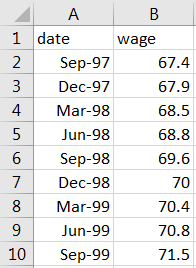
\includegraphics{2018sem2_q2_1}}
\end{figure}
\vspace{-\baselineskip} \noindent Save the CSV file and read it in EViews. Note that EViews automatically realises that you have quarterly data.

\noindent \textcolor{red}{1. Plot the $wage$ series (plotting a time series means producing a line plot of the series in which the x-axis is time. In EViews, clicking on a series opens a window that shows the values of the series in a spreadsheet. This window has a menu bar. Under $View$ is $Graph$ and the default graph is a line plot.) What can we learn from this plot?}

\noindent Double click on $wage$,
\begin{figure}[H]
	\centerline{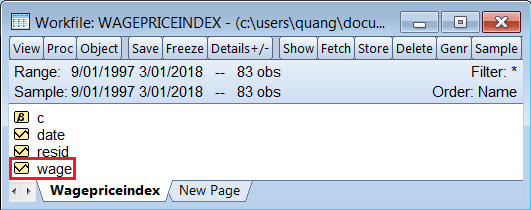
\includegraphics{2018sem2_q2_2}}
\end{figure}
\vspace{-\baselineskip} \noindent then, $$View \to Graph$$
\begin{figure}[H]
	\centerline{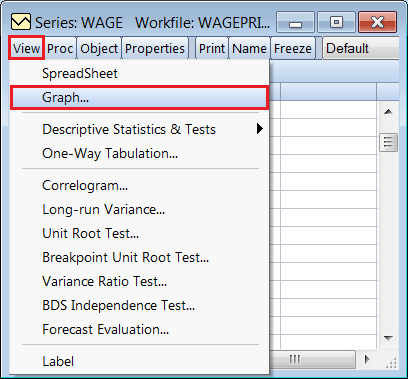
\includegraphics{2018sem2_q2_3}}
\end{figure}
\vspace{-\baselineskip} $$Specific: Line\ \&\ Symbol$$
\begin{figure}[H]
	\centerline{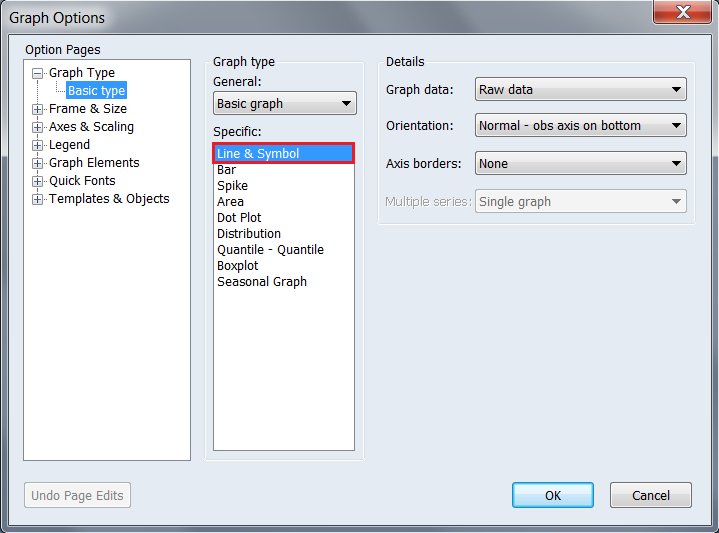
\includegraphics{2018sem2_q2_4}}
\end{figure}
\vspace{-\baselineskip}
\begin{figure}[H]
	\centerline{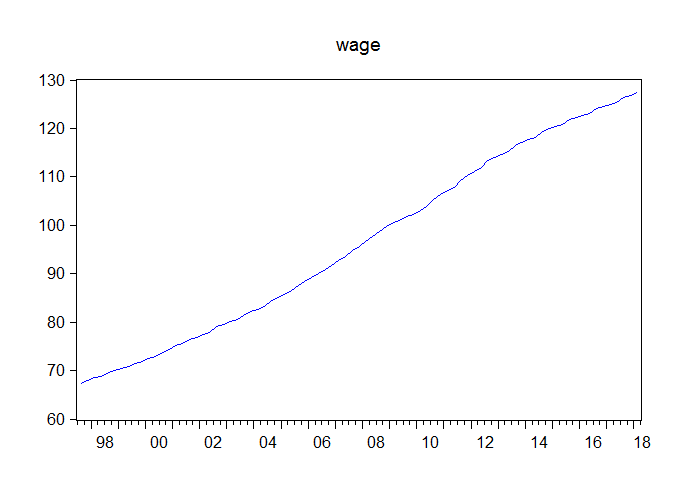
\includegraphics{wageline}}
\end{figure}
\vspace{-\baselineskip} 
\justify
\begin{blueframed}
	\textcolor{blue}{\textbf{Background}}
	\vspace{-\baselineskip}
	\justify
	\textcolor{blue}{\underline{Trends and seasonality}}
	
	\noindent \textcolor{blue}
	{
		A persistent downward or upward movement, often over 10+ years, indicates that there is a $trend$ in the time series. If we observe fluctuations within a one-year period that repeats in the same fashion year-after-year, then the time series exhibits $seasonality$.
	}
\end{blueframed} \noindent From the line graph of hourly wage, we observe an upward trend i.e. hourly wage increases with time. Hourly wage is also highly persistent as each observation is very close to observations before it.

\noindent \textcolor{red}{2. If we were interested in forecasting hourly wage in the next period, would sample average be a good forecast? Suggest more appropriate forecast.}

\noindent No, the sample mean of hourly wage would not be a good forecast of hourly wage in the next period because the mean increases with time. For example, the mean hourly wage index in 2017 is higher than the mean in 2016, 2015, etc. and the mean hourly wage index in 2016 is higher than the mean in 2015, 2014, etc.
\begin{figure}[H]
	\centerline{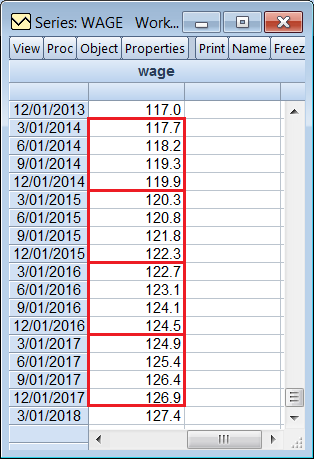
\includegraphics{2018sem2_q2_5}}
\end{figure}
\vspace{-\baselineskip} \noindent We could use the previous observation of hourly wage as a forecast of hourly wage in the coming period but there are many better approaches. Another example is to base the next quarter's growth on an average quarter on quarter growth of hourly wage of the same quarters.
\begin{itemize}
	\item Forecasting hourly wage in 2018 quarter 2.
	\item Compute average growth from quarter 1 to quarter 2.
	\item Assume quarterly growth from 2018 quarter 1 to 2018 quarter 2 is the same as the average growth from quarter 1 to quarter 2.
	\item $forecast\_2018\_quarter\_2 = 2018\_quarter\_1 \times (1 + average\_growth\_Q1\_to\_Q2)$
\end{itemize}

\noindent \textcolor{red}{3. Generate the growth rate of hourly wage using the log-returns formula. 
\begin{align*}
	g_t &= 100 \times \Delta log(wage_t) \\
	&= 100 \times (log(wage_t) - log(wage_{t-1}))
\end{align*}
EViews has a built in function `dlog(X)' which computes the difference of logarithm of X. Open this series. Why is the first value of this series NA?}

\noindent To generate the growth rate of hourly wage using the log-returns formula in EViews click $Genr$,
\begin{figure}[H]
	\centerline{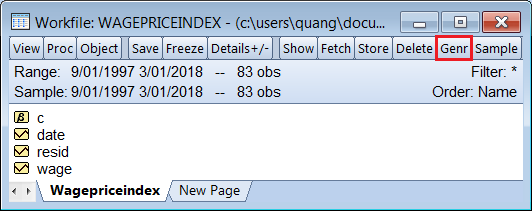
\includegraphics{2018sem2_q2_7}}
\end{figure}
\vspace{-\baselineskip}
$$Enter\ Equation: wage\_growth = 100^*dlog(wage)$$
\begin{figure}[H]
	\centerline{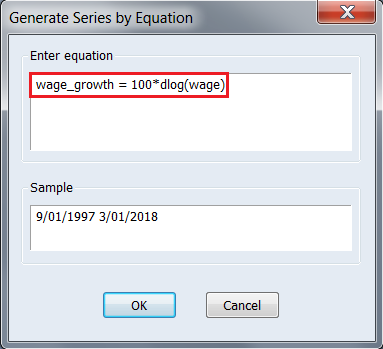
\includegraphics{2018sem2_q2_6}}
\end{figure}
\vspace{-\baselineskip}
\begin{figure}[H]
	\centerline{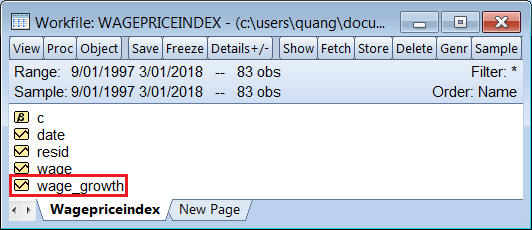
\includegraphics{2018sem2_q2_8}}
\end{figure}
\vspace{-\baselineskip}
\begin{figure}[H]
	\centerline{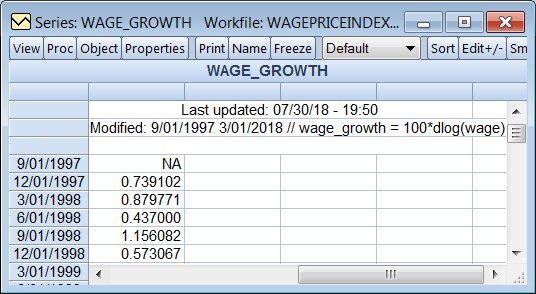
\includegraphics{2018sem2_q2_9}}
\end{figure}
\vspace{-\baselineskip} \noindent The first value in this series is the growth rate of hourly wage in 1997 quarter 3 and is $NA$ because we require hourly wage in 1997 quarter 2 to compute this value, which we do not have. \begin{align*}
wage\_growth_t &= 100 \times (log(wage_t) - log(wage_{t-1})) \\
wage\_growth_{1997Q3} &= 100 \times (log(wage_{1997Q3}) - log(wage_{1997Q2})) \\
&= 100 \times (log(67.4) - log(wage_{1997Q2}))
\end{align*}
\begin{figure}[H]
	\centerline{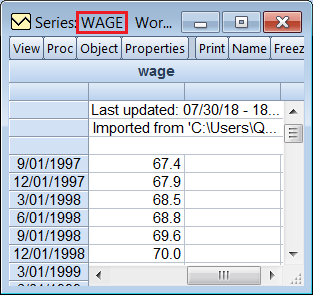
\includegraphics{2018sem2_q2_10}}
\end{figure}

\newpage
\noindent \textcolor{red}{4. Plot the growth rate of wage. What does this plot tell you?}

\noindent Open $wage\_growth$, \begin{figure}[H]
	\centerline{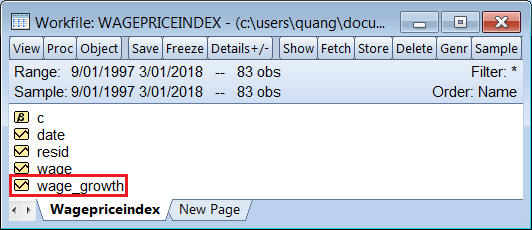
\includegraphics{2018sem2_q2_8}}
\end{figure}
\vspace{-\baselineskip} then $$View \to Graph$$ \begin{figure}[H]
	\centerline{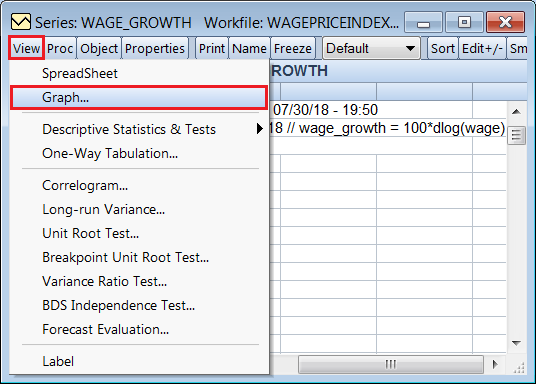
\includegraphics{2018sem2_q2_11}}
\end{figure}
\vspace{-\baselineskip} $$Specific: Line\ \&\ Symbol$$
\begin{figure}[H]
	\centerline{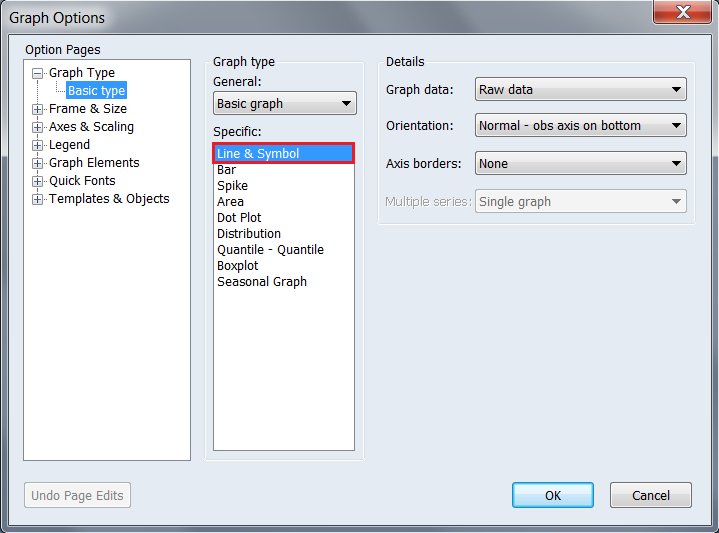
\includegraphics{2018sem2_q2_4}}
\end{figure}
\vspace{-\baselineskip}
\begin{figure}[H]
	\centerline{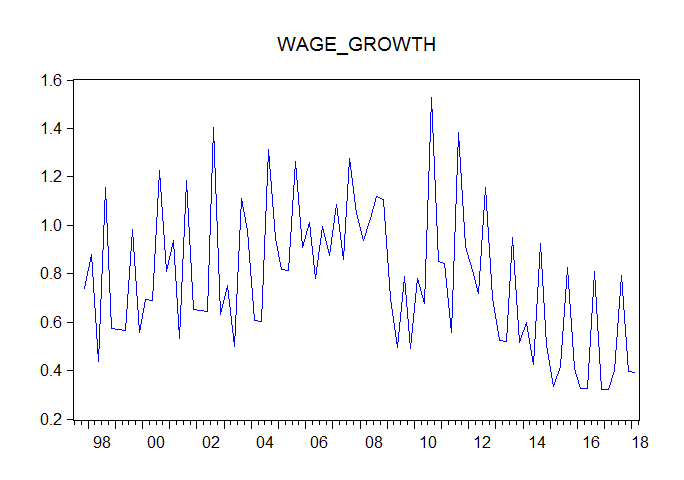
\includegraphics{wagegrowthline}}
\end{figure}
\vspace{-\baselineskip} \noindent There is clear seasonality in the growth rate of hourly wage i.e growth rate of hourly wage is highest in the 3rd quarter of each year. This may be due to the fact that most people's wage increases become effective at the beginning of the financial year.

\noindent \textcolor{red}{5. Look at the seasonal plots of the growth rate of wage. To plot seasonal plots of $wage\_growth$, open $wage\_growth$, \noindent Open $wage\_growth$, \begin{figure}[H]
		\centerline{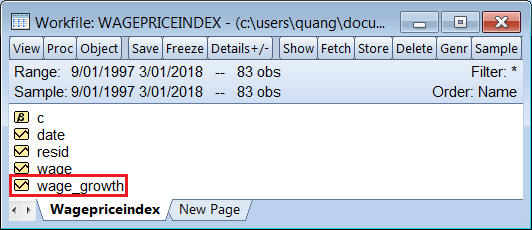
\includegraphics{2018sem2_q2_8}}
	\end{figure}
	\vspace{-\baselineskip} then $$View \to Graph$$ \begin{figure}[H]
		\centerline{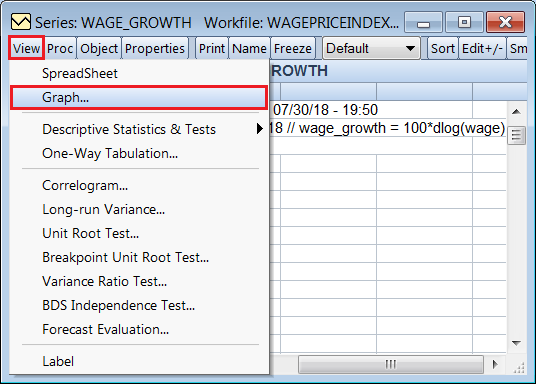
\includegraphics{2018sem2_q2_11}}
	\end{figure}
	\vspace{-\baselineskip} $$Specific: Seasonal\ Graph \quad Seasonal\ type: Paneled\ lines\ \&\ means$$\begin{figure}[H]
		\centerline{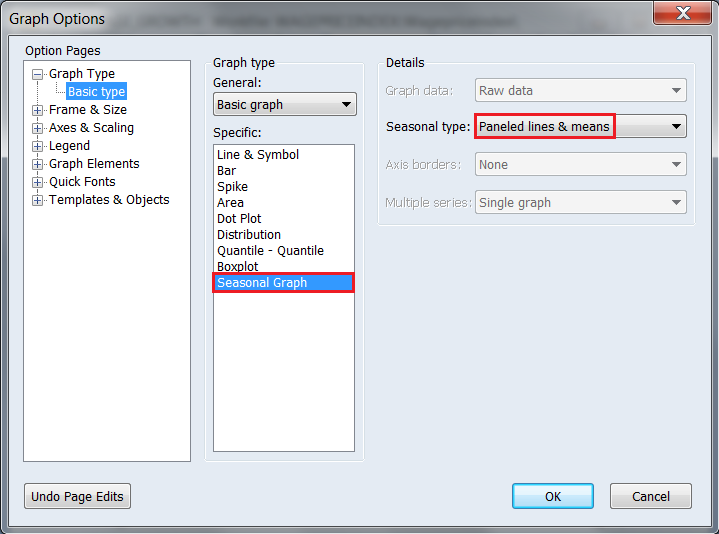
\includegraphics{2018sem2_q2_12}}
	\end{figure}
	\vspace{-\baselineskip}}
\begin{figure}[H]
	\centerline{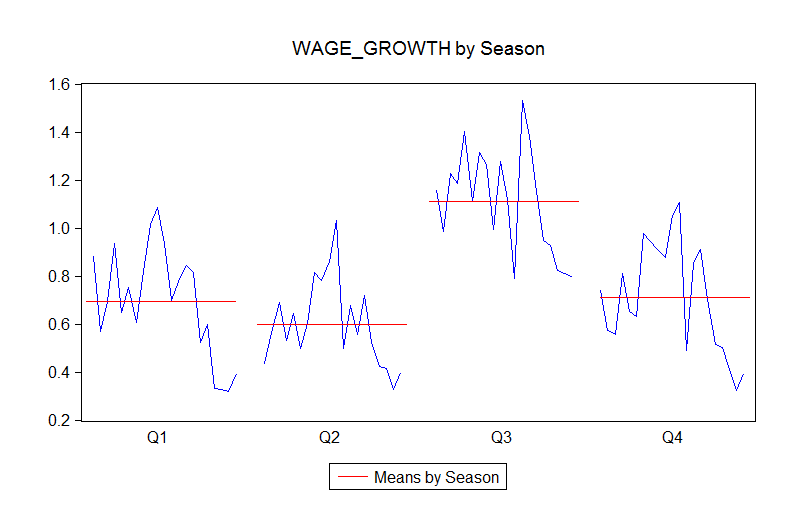
\includegraphics{wageseasongraph}}
\end{figure}
\vspace{-\baselineskip}
\begin{figure}[H]
	\centerline{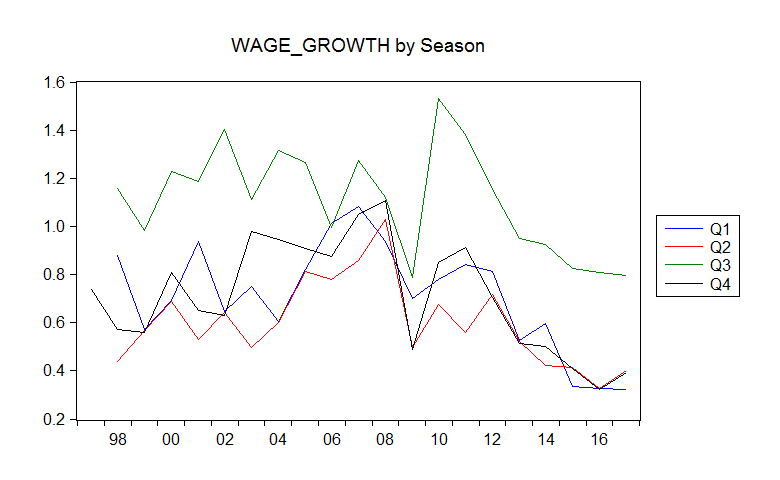
\includegraphics{multipleoverlaylines}}
\end{figure}
\vspace{-\baselineskip}

\noindent Wage growth in the 3rd quarter is higher than in other quarters.

\noindent \textcolor{red}{6. Look at the time series plot of the growth rate of wage again. Mentally adjust for seasonal variation. Do you see that wage growth has been declining since 2010? Should that by itself worry us? What else do we need if we are worried about the value of one hour of work?}
\begin{itemize}
	\item These wages are nominal wages which have not been adjusted for inflation.
	\item Real wage is adjusted for inflation and represents how much we can buy with our wage.
	\item If nominal wage growth is lower but inflation is lower as well, then real wage growth could be lower, steady, or higher, depending on the relative magnitude of nominal growth rate and inflation rate.
	\item  Suppose your nominal wage increases, but inflation increases at a rate that is greater than your wage increase. In this instance, your purchasing power has weaken because although your wage has increased the price of goods \& services has increased proportional greater than your wage. 
	\item We need to look at the inflation rate to determine what happened to real growth rate.
\end{itemize}



\end{document}
